\subsection{Нормална Форма на Чомски}
\index{Чомски}
%[стр. 99 от \cite{sipser}]
\index{нормална форма на Чомски}
Една безконтекстна граматика е в {\bf нормална форма на Чомски}, ако
всяко правило е от вида
\[A \rightarrow BC\mbox{ и }A \rightarrow a,\]
където $A, B, C$ са произволни променливи и $a$ е произволна буква.
\mynote{Ако искаме $\varepsilon$ да бъде в езика на граматиката, то позволяваме от началната променлива $S$ да имаме правилото $S \to_G \varepsilon$,
но тогава забраняваме $S$ да се среща в дясна страна на правило.}
% Освен това, позволяваме правилото $S\to\varepsilon$.
% \footnote{В \cite[стр. 151]{papadimitriou} дефиницията е малко по-различна.
% Там дефинират $G$ да бъде в нормална форма на Чомски ако $R \subseteq V\times(V\cup\Sigma)^2$.
% В този случай губим езиците $\{\varepsilon\}$ и $\{a\}$, за $a\in\Sigma$.}

\begin{framed}
  \begin{theorem}
    Всеки безконтекстен език $L$, който не съдържа $\varepsilon$, се поражда от безконтекстна граматика в нормална форма на Чомски.
  \end{theorem}
\end{framed}
\begin{proof}
%  \marginpar{Броят на правилата може да се увеличи експоненциално.}
  Нека имаме безконтекстна граматика $G$, за която $L = \L(G)$.
  Ще построим безконтекстна граматика $G^\prime$ в нормална форма на Чомски, $L = \L(G^\prime)$.
  % [стр. 99 от \cite{sipser}]
  Следваме следната процедура:
  \begin{itemize}
  \item
    Премахваме дългите правила.
    Това можем да направим за време $\mathcal{O}(|G|)$
    като новата граматика ще има дължина $\mathcal{O}(|G|)$.
  \item
    \mynote{Редът на стъпките е важен. Трябва преди това сме премахнали дългите правила. Вижте \cite[стр. 296]{hopcroft2}.}
    Премахваме $\varepsilon$-правилата.
    Това можем да направим за време $\mathcal{O}(|G|^2)$
    като новата граматика ще има дължина $\mathcal{O}(|G|)$.
  \item
    Премахваме преименуващите правила.
    Това можем да направим за време $\mathcal{O}(|G|^2)$
    като новата граматика ще има дължина $\mathcal{O}(|G|^2)$.
  \item
    За правила от вида $A\to u_1 u_2$, където $u_1, u_2 \in V \cup \Sigma$, 
    заменяме всяка буква $u_i$ с новата променлива $U_i$
    и добавяме правилото $U_i\to u_i$.
    Например, правилото $A \to aB$ се заменя с правилото $A \to XB$ и добавяме правилото $X \to a$,
    където $X$ е нова променлива.
    Това можем да направим за време $\mathcal{O}(|G|)$ и новата граматика ще има дължина $\mathcal{O}(|G|)$.
  \item
    Ако искаме $\varepsilon$ да бъде в езика на граматиката, то добавяме нова начална променлива $S_0$
    и правило $S_0 \to_G \varepsilon$ и правилата $S_0 \to \alpha$ за $S \to \alpha$.
  \end{itemize}
\end{proof}

\begin{theorem}
  При дадена безконтекстна граматика $G$, можем да намерим еквивалентна
  на нея граматика $G'$ в нормална форма на Чомски за време $\mathcal{O}(|G|^2)$,
  като получената граматика е с дължина $\mathcal{O}(|G|^2)$.
\end{theorem}

\begin{theorem}
  \mynote{\cite[стр. 137]{hopcroft1}. Важно е, че алгоритмът е полиномиален.
    \writedown Защо от \Lemma{pumping-context} имаме експоненциален алгоритъм за проверка дали езикът на една граматика е безкраен?}
  Съществува \emph{полиномиален} алгоритъм, който определя по дадена безконтекстна граматика $G$ дали $\L(G)$ е безкраен език.
\end{theorem}
\begin{proof}
  Нека е дадена една безконтекстна граматика $G$.
  Нека да разгледаме граматиката $G'$ в НФЧ {\em без безполезни променливи}, за която $\L(G) = \L(G')$.
  От граматиката $G' = \pair{V',\Sigma,S,R'}$ строим граф с възли променливите от $V'$ като
  за $A,B \in V'$ имаме ребро $A \to B$ в графа точно тогава, когато съществува $C \in V'$,
  за което $A \to_{G'} BC$ или $A \to_{G'} CB$ е правило в граматиката $G$.
  Сега ще съобразим, че ако в получения граф имаме цикъл, то $\L(G') = \infty$.
  Да разгледаме един такъв цикъл в графа:
  \[A_0 \to A_1 \to A_2 \to \cdots \to A_n \to A_0.\]
  Понеже граматиката е в нормална форма на Чомски, то същестуват думи $\lambda,\rho \in (V\cup\Sigma)^\star$, за които $A_0 \yield{n+1} \lambda A_0 \rho$ и $\abs{\lambda\rho} = n+1$

  \begin{figure}[H]
    \begin{subfigure}[t]{0.5\textwidth}
    \centering
      \begin{tikzpicture}[scale=0.8]
      \node (A) at (0,0) {\footnotesize{$A_0$}};
      \coordinate (B) at (-2,-3);
      \coordinate (C) at (2,-3);
      \node (D) at (0,-1.2) {\footnotesize{$A_i$}};
      \coordinate (D1) at (1.4,-3);
      \coordinate (D2) at (-1.4,-3);
      \node (E) at (0,-2.3) {\footnotesize{$A_n$}};
      \coordinate (E1) at (0.7,-3);
      \coordinate (E2) at (-0.7,-3);
      \coordinate (F) at (0,-3);

      \draw (A) -- node[above left]{$P = $} (B) -- node[below]{$A_0$}(C) -- (A);
      \draw [photon] (A) -- (D) -- (E) -- (F);
    \end{tikzpicture}
    \caption{$A_0 \yield{n+1} \lambda A_0 \rho$, където $\lambda, \rho \in (V\cup\Sigma)^\star$.}
    \end{subfigure}
    ~ 
    \begin{subfigure}[t]{0.5\textwidth}
      \centering
      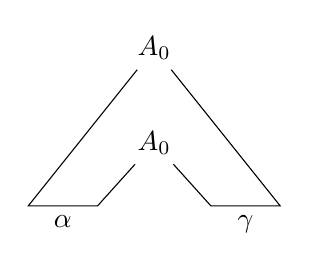
\begin{tikzpicture}[scale=0.8]
        \node (A) at (0,0) {$A_0$};
        \coordinate (B) at (-2,-2.5);
        \coordinate (C) at (2,-2.5);
        \coordinate (D) at (-0.9,-2.5);
        \coordinate (E) at (0.9,-2.5);
        \node (F) at (0,-1.5) {$A_0$};
        \draw (A) -- (B) -- node[below]{$\alpha$} (D) -- (F) -- (E) -- node[below]{$\gamma$} (C) -- (A);
      \end{tikzpicture}
      \caption{$A_0 \yield{\geq n+1}\alpha A_0\gamma$, където $\alpha,\gamma \in \Sigma^\star$.}
    \end{subfigure}
  \end{figure}

  Понеже в $G$ няма безполезни променливи, то $\lambda \derive{\star} \alpha$, където $\alpha \in \Sigma^\star$ и $\abs{\lambda} \leq \abs{\alpha}$ и $\rho \derive{\star} \gamma$,
  където $\gamma \in \Sigma^\star$ и $\abs{\rho} \leq \abs{\gamma}$.
  Оттук заключаваме, че $A_0 \yield{\star} \alpha A_0 \gamma$ и $\abs{\alpha\gamma} \geq 1$.
  Понеже $A_0$ не е безполезна променлива, то $A_0 \yield{\star} \beta$, за някоя дума $\beta \in \Sigma^\star$.
  Сега комбинираме \Proposition{pumping:ground} и \Proposition{pumping:iteration} за да получим следния извод:
  \begin{prooftree}
    \AxiomC{$A_0 \yield{\star} \alpha A_0 \gamma$}
    \AxiomC{$A_0 \yield{\star} \beta$}
    \AxiomC{$i \in \Nat$}
    \TrinaryInfC{$A_0 \yield{\star} \alpha^i \beta \gamma^i$}
  \end{prooftree}
  Понеже $\abs{\alpha\beta} \geq 1$, заключаваме, че $\L(G)$ е безкраен език.
  Така доказахме, че ако в графът има цикли, то $\L(G)$ е безкраен език.
  
  За обратната посока, нека в графът няма цикли.
  Да разгледаме една променлива $A$, от която най-дългият път има $k$ на брой възли.
  От принципа на Дирихле знаем, че $k \leq \abs{V}$.
  Това означава, че ако $A \yield{\star} \alpha$, за някоя $\alpha \in \Sigma^\star$,
  то $A \yield{\leq k} \alpha$ и понеже граматиката е в нормална форма на Чомски,
  то $\abs{\alpha} \leq 2^{k-1}$.
  Оттук следва, че всички думи, които се извеждат от променливата $A$ са най-много $2^{k-1}$ на брой.
  Заключаваме, че ако в графът няма цикли, то $\L(G)$ е краен.
\end{proof}

\begin{theorem}
  Съществува \emph{полиномиален} алгоритъм, който определя по дадена безконтекстна граматика $G$ дали $\L(G)$ е краен език.
\end{theorem}

%%% Local Variables:
%%% mode: latex
%%% TeX-master: "../eai"
%%% End:
